\chapter{LHC and the CMS experiment}
\chaptermark{The LHC and the CMS experiment}  
\thispagestyle{plain}  % First page has default style
\pagestyle{chapterpages}
\label{Section:Chapter3}

The physics analyses presented in this thesis are performed using data generated by the LHC and collected by the \ac{CMS} experiment. This chapter begins by exploring how the LHC accelerates and collides protons up to centre-of-mass energies ($\sqrt{s}$) of $13.6\TeV$, creating the extreme but necessary conditions needed for rigorous tests of the SM at the electroweak scale. The discussion then shifts to the CMS detector, a multipurpose apparatus composed of several layers of specialised subdetectors. These intricate systems work in concert to enable the precise reconstruction of particles emerging from proton-proton collisions at the heart of the detector.

\section{The LHC}

The LHC~\cite{LHC_1}, situated at the \ac{CERN} near Geneva, Switzerland, is a testament to human scientific achievement. Ingeniously, the LHC was placed within the tunnel previously occupied by the \ac{LEP} collider. Engineered to facilitate proton-proton (pp) collisions, the machine was designed to generate such collisions with centre-of-mass energy up to $14\TeV$ and an unprecedented luminosity of $10^{34}\unit{cm}^{-2}\unit{s}^{-1}$. As mentioned earlier, the LHC is currently running just below its maximum energy capabilities, with each beam carrying $6.8\TeV$ of energy. Spanning a circumference of $27\unit{km}$, the LHC mirrors the basic layout of its predecessor, LEP, as illustrated in Fig~\ref{Figure:Chapter3_LHC_BasicLayout}. 

\begin{figure}[h]
\centering
\includegraphics[width= 0.7\textwidth]{Figures/Chapter3/LHC_BasicLayout.jpg}
\caption{Basic schematic layout of the LHC consisting of 8 arc sections along with the two circulating beams. The locations of the ATLAS, ALICE, CMS, and LHCb experiments are also displayed. Figure taken from Ref.~\cite{LHC_BasicLayout}.}
\label{Figure:Chapter3_LHC_BasicLayout}
\end{figure}

The experimental landscape is strategically arranged with two general-purpose experiments, ATLAS~\cite{LHC_ATLAS} and CMS~\cite{LHC_CMS}, positioned at diametrically opposite sections, at Points 1 and 5 respectively. The ALICE experiment~\cite{LHC_ALICE} occupies Point 2, while LHCb~\cite{LHC_LCHb} is situated at Point 8. At these critical locations, the circulating beams are precisely focused and brought into collision.

Particles are not accelerated to an energy of $6.8\TeV$ per beam simply by circulating in the LHC tunnel. Instead, the LHC is the final stage of a sophisticated accelerator chain~\cite{LHC_InjectorComplex} at CERN, in which a series of machines successively boost the energy of the particles, as shown in Fig.~\ref{Figure:Chapter3_LHC_Complex}. The first step in this accelerator complex is the \textbf{\ac{LINAC4}}~\cite{LINAC4}, which produces a beam of negative hydrogen ions ($\text{H}^-$), each consisting of a proton and two electrons. LINAC4 accelerates these ions to an energy of $160\MeV$ before injecting them into the \textbf{\ac{PSB}}. During injection, the electrons are stripped off, leaving behind bare protons. The PSB then accelerates the protons to a kinetic energy of $2.0\GeV$. Next, the beam is transferred to the \textbf{\ac{PS}}, which increases its energy to $26\GeV$. From there, the particles are sent to the largest machine in the injector complex, the \textbf{\ac{SPS}}, which boosts their energy to $450\GeV$. Throughout the injector chain, the protons are grouped into bunches, which are subsequently injected into the two concentric beam pipes of the LHC as two counter-rotating beams. The injection continues until each beam consists of 2,808 bunches, separated by $25\unit{ns}$.

\begin{figure}[h]
\centering
\includegraphics[width= 1.0\textwidth]{Figures/Chapter3/LHC_AcceleratorComplex.png}
\caption{Schematic diagram of the CERN accelerator complex. Figure taken from Ref.~\cite{LHC_InjectorComplex}.}
\label{Figure:Chapter3_LHC_Complex}
\end{figure}

A network of 1,232 superconducting (niobium-titanium) dipole magnets bends the beams along the circular LHC ring. These magnets operate at ultra-low temperatures of $1.9\unit{K}$, achieved using superfluid helium, and can produce magnetic fields up to $8.4\unit{T}$. Beam acceleration is facilitated by sixteen $400\unit{MHz}$ radiofrequency (RF) cavities, providing a $\sim\!14$-fold energy increase compared to the injection energy. The circular trajectory of the accelerating beams is maintained by dynamically adjusting the magnetic field strength of the dipole magnets, while 392 quadrupoles are utilised to focus the beams. Just before the collision at each of the four principal points, four inner triplet quadrupole magnets are used to reduce the transverse size of the beams. This effectively squeezes them, aiming to maximise the collision rate~\cite{LHC_Run3}. The specifications mentioned above reflect the state of the accelerator complex following the upgrades carried out during the latest scheduled long shutdown, which was completed in 2021.

\subsection{Cross section and Luminosity}

Cross section and luminosity are essential in understanding and measuring what happens in collider collisions. Together, these determine how often specific physical processes occur in the detector. The cross-section ($\sigma$) describes the probability of a particular process occurring during a collision. Many different processes can occur as the beams cross in the heart of the LHC detectors. The cross-section of each of these processes depends on the type and the energy of the colliding particles, $\sigma(\sqrt{s})$. The cross-section is combined with the instantaneous luminosity ($\mathscr{L}$) to calculate how often a particular process occurs at a collider. Instantaneous luminosity is a measure of how tightly particles are packed into a given space, and it is a function of the beam parameters~\cite{LHC_HL},

\begin{equation}
\begin{aligned}
    \mathscr{L} &= \gamma \frac{n_b N^2 f_{\text{rev}}}{4\pi \beta^* \epsilon_n} R \\
    R &= 1 / \sqrt{1 + \left( \frac{\theta_c \sigma_z}{2\sigma} \right) }
\end{aligned}
\end{equation}

where $\gamma$ is the proton beam energy expressed in rest mass units, $n_b$ is the number of bunches per beam, $N$ is the number of particles per bunch, $f_{rev}$ is the revolution frequency ($11.2\unit{kHz}$), $\beta^*$ is the beam beta function at the collision point and $\epsilon_n$ is the normalised transverse beam emittance. The term R is a geometrical reduction factor for luminosity. This is expressed as a function of the crossing angle of the beams at the collision point ($\theta_c$) and the transverse (longitudinal) spread of the particle bunch, $\sigma_z(\sigma)$. 

The cross-section, together with the instantaneous luminosity, determines the rate (R) at which a given process occurs in the detector,

\begin{equation}
    R = \sigma(\sqrt{s}) \cdot \mathscr{L} 
\end{equation}

The luminosity is not static, as it depends on beam parameters that change over time. In this case, a more appropriate quantity is the integrated luminosity ($\mathscr{L}_{int}$), which considers the total data collected over a given period,

\begin{equation}
    \mathscr{L}_{int} = \int \mathscr{L}(t) dt
\end{equation}

In a given period, the total number of events (N) for a particular process with cross-section $\sigma$ can be expressed as:

\begin{equation}
    \mathscr{N} = \sigma \cdot \mathscr{L}_{int}
\end{equation}

A summary of the total integrated luminosity delivered to the CMS experiment since 2015 is provided in Fig.~\ref{Figure:Chapter3_CMS_IntegratedLumi}.

\begin{figure}[h]
\centering
\includegraphics[width= 0.7\textwidth]{Figures/Chapter3/CMS_IntegratedLumi.pdf}
\caption{Total integrated luminosity delivered to the CMS experiment between 2015 and 2024. Data collected from all periods except 2015 and 2024 are used in this thesis. Figure taken from Ref.~\cite{CMS_IntegratedLumi}.}
\label{Figure:Chapter3_CMS_IntegratedLumi}
\end{figure}

\subsection{Pileup}

The CMS experiment set out to investigate the rarest interactions of proton collisions. In the effort of maximising the chances of observing such rare events, the LHC collides large bunches of protons rather than single protons, as discussed earlier. This approach increases the instantaneous luminosity, which is favourable because it directly enhances the probability of rare processes occurring within a given time. However, this also introduces challenges: when bunches collide, multiple protons interact simultaneously. In other words, CMS records particles from the interaction of interest and particles originating from multiple additional interactions, called \ac{PU} interactions. Increasing the instantaneous luminosity leads to an enhancement of PU, and removing these unwanted overlap collisions requires increasingly sophisticated techniques. Figure~\ref{Figure:Chapter3_CMS_Pileup} illustrates the PU conditions encountered by the CMS experiment between 2015 and 2024.

\begin{figure}[h]
\centering
\includegraphics[width= 0.7\textwidth]{Figures/Chapter3/CMS_Pileup.pdf}
\caption{Distribution of the average number of interactions per bunch crossing for pp collisions between 2015 to 2024, using data from the CMS experiment. Figure taken from Ref.~\cite{CMS_IntegratedLumi}.}
\label{Figure:Chapter3_CMS_Pileup}
\end{figure}

\section{The CMS Detector}
\label{Section:Chapter3_CMS_Detector_Introduction}
As previously discussed, CMS is one of the two general-purpose detectors at the LHC, built to explore a wide range of high-energy physics phenomena. The design of the CMS detector was shaped by the ambitious goals of the LHC physics programme~\cite{LHC_CMS}, which demanded precise and efficient measurements under challenging experimental conditions. To accomplish these objectives, several key performance requirements were identified:

\begin{itemize}
  \item Identification \& precise momentum reconstruction of muons over a broad range of momenta and angles; dimuon mass resolution $\sim1\%$ at $100\GeV$; unambiguous muon charge identification up to $1\TeV$
  \item High momentum resolution \& reconstruction efficiency for charged particles; efficient $\tau$‐lepton and b‐jet identification
  \item Photon/electron energy measurement with excellent resolution; diphoton and dimuon mass resolution $\sim1\%$ at $100\GeV$ over a wide geometrical coverage
  \item Effective $\pi^0$ rejection; efficient isolation of photons and leptons in high‐luminosity, high‐occupancy conditions
  \item Precise dijet mass reconstruction and MET resolution
\end{itemize}

CMS employs a compact, layered detector system arranged cylindrically around the interaction point to fulfil these performance requirements, providing a near-complete solid-angle coverage. The entire detector is $21.6\unit{m}$ long and has a diameter of $14.6\unit{m}$ while weighing $12,500\unit{t}$. This makes CMS one of the largest yet compact detectors ever engineered for a particle physics experiment. Closest to the beam pipe lies the \textbf{silicon tracker}, which precisely tracks charged particles. It is surrounded by the \textbf{\ac{ECAL}}, optimised for measuring the energy of electrons and photons with high precision. The \textbf{\ac{HCAL}} follows and is responsible for absorbing and measuring the energy of hadrons. These three subsystems are enclosed within a powerful $13\unit{m}$ long, $6\unit{m}$ inner-diameter, $3.8\unit{T}$ \textbf{superconducting solenoid}. Embedded within the iron return yoke of the solenoid is the \textbf{muon detection system}. A schematic of the full CMS detector is shown in Fig.~\ref{Figure:Chapter3_CMS_schematic}, providing an overview of its cylindrical geometry and layered structure around the LHC interaction point. The following sections will provide a more detailed discussion of each of the major detector subsystems introduced here. A complementary longitudinal slice through the detector is shown in Fig.~\ref{Figure:Chapter3_CMS_slice}, serving as a visual reference for the detailed subsystem descriptions that follow.

\begin{figure}[h]
\centering
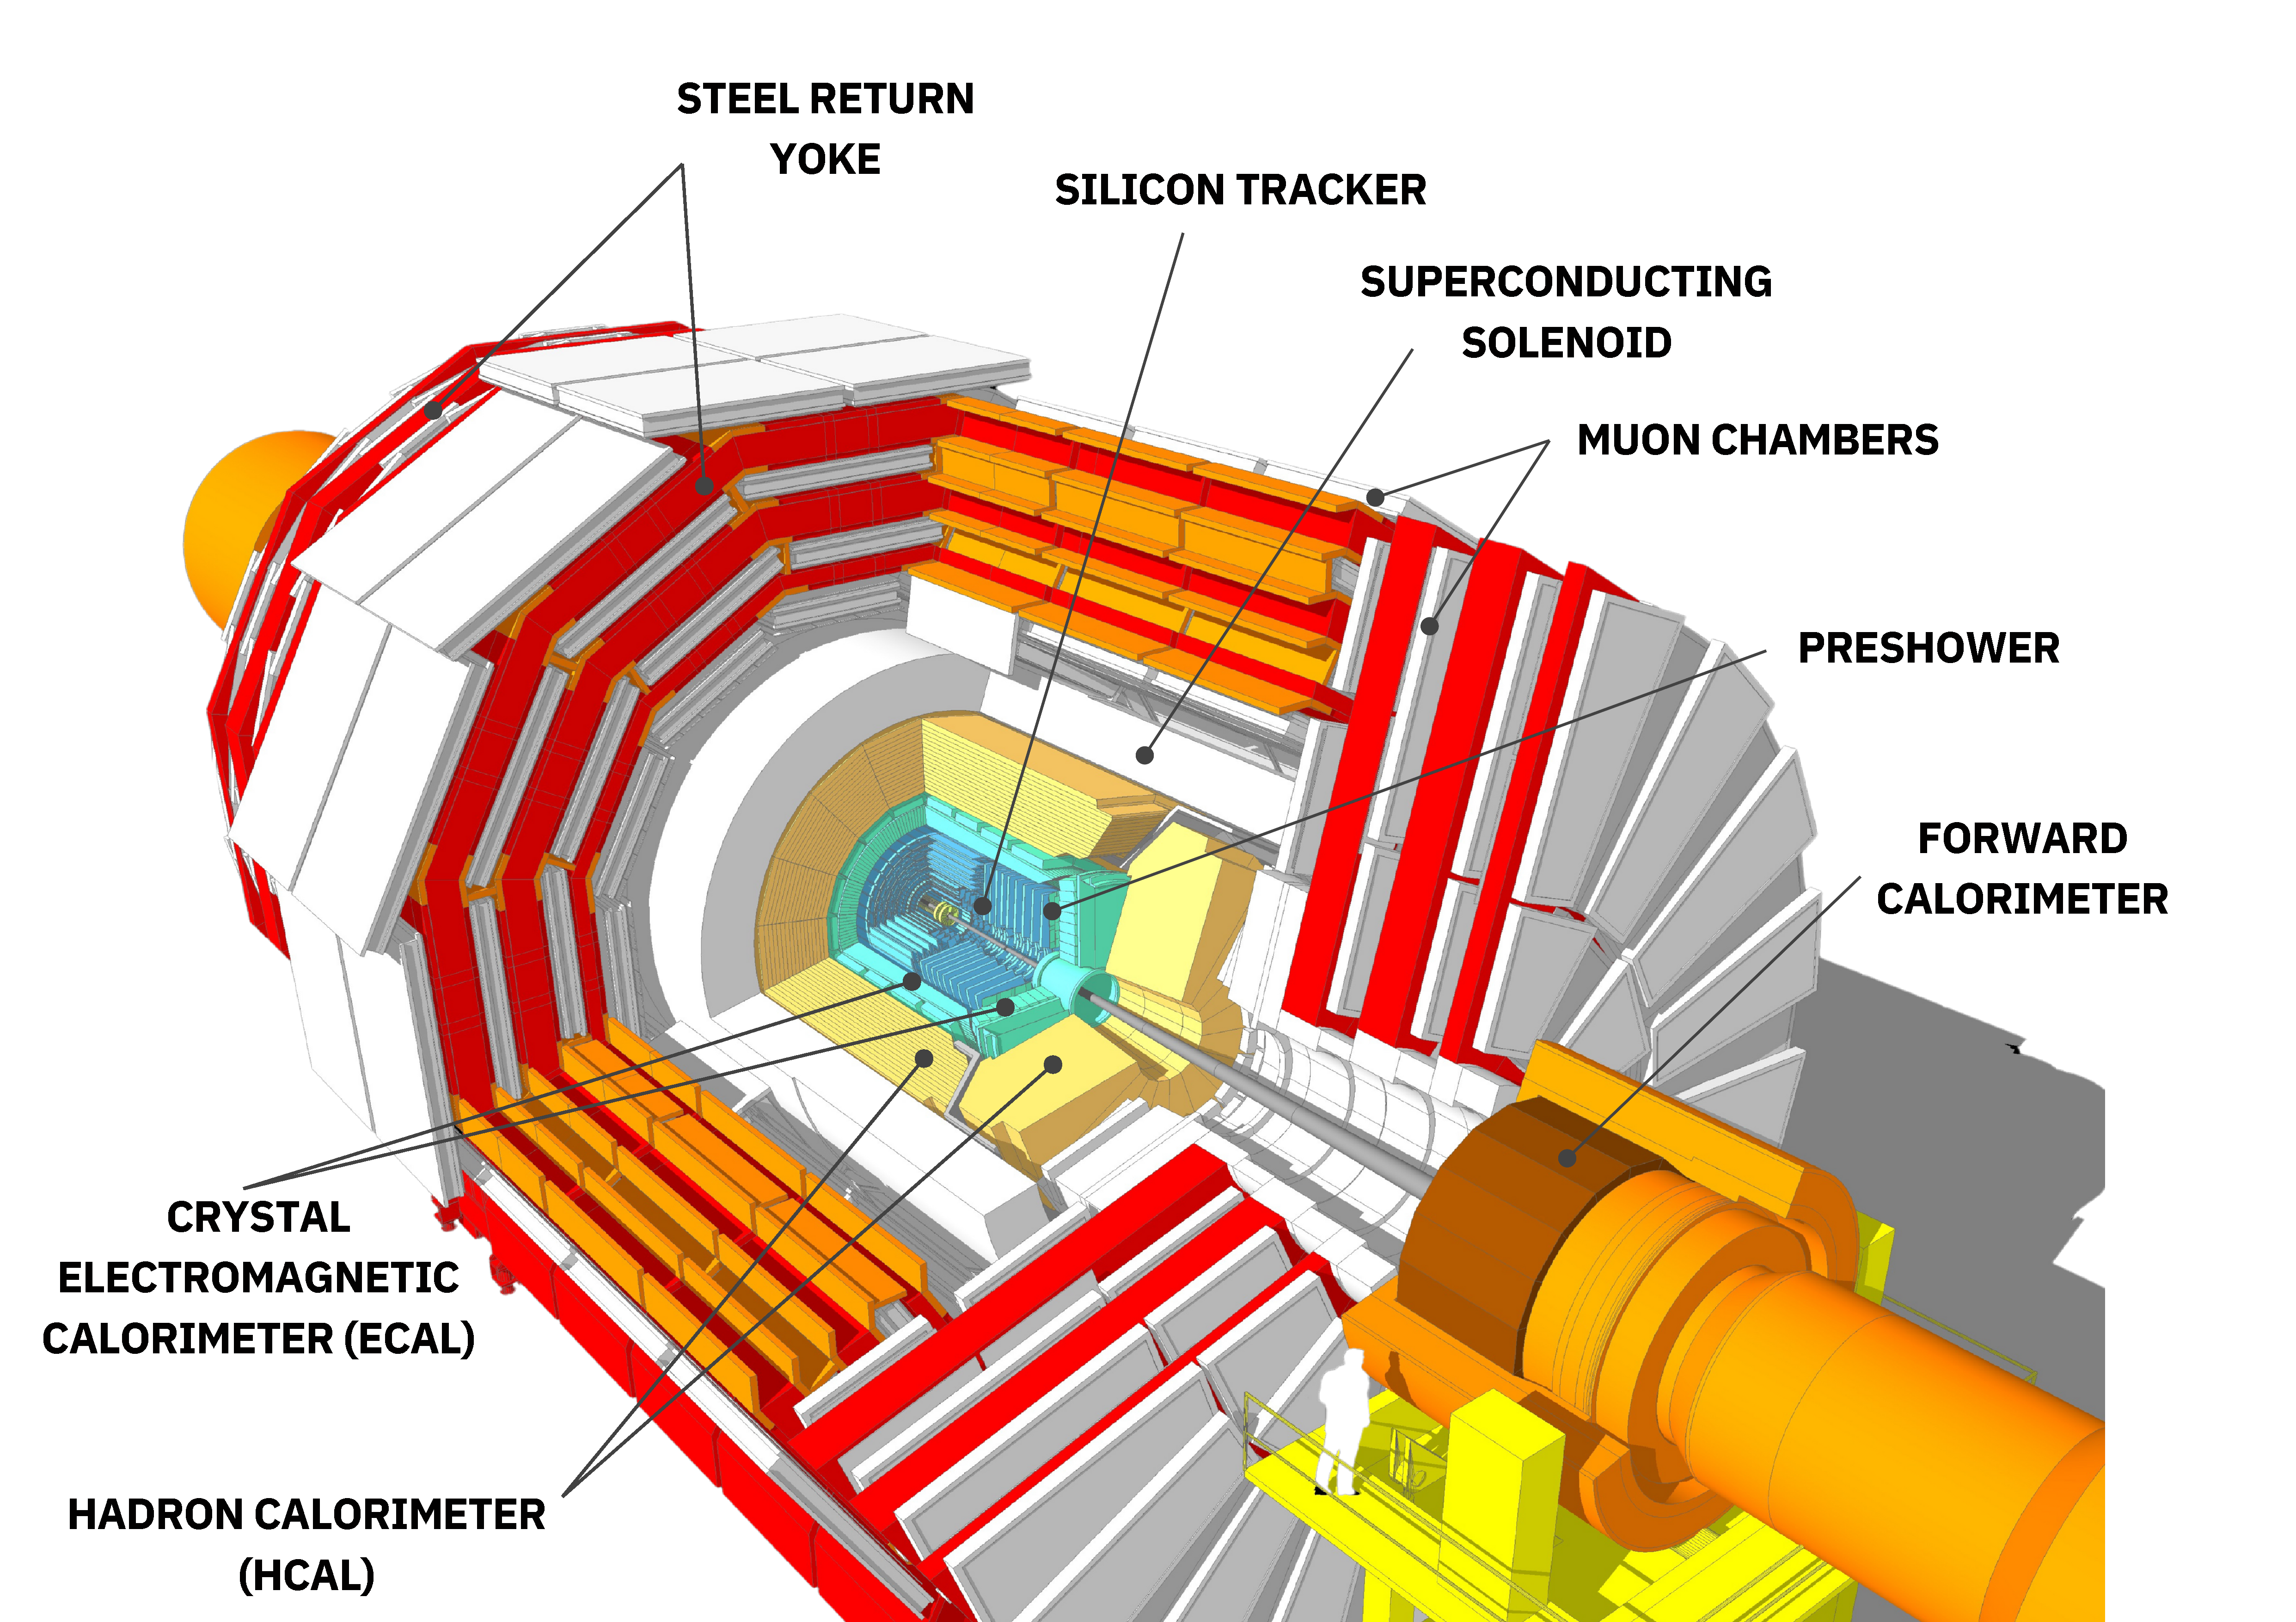
\includegraphics[width= 1\textwidth]{Figures/Chapter3/CMS_Detector.png}
\caption{Schematic drawing of the CMS detector. Figure taken from Ref.~\cite{CMS_Detector_Run3}.}
\label{Figure:Chapter3_CMS_schematic}
\end{figure}

\begin{figure}[h]
\centering
\includegraphics[width= 1\textwidth]{Figures/Chapter3/CMS_Detector_Slice.pdf}
\caption{A transverse slice of the CMS detector displaying the individual subsystems and their response to different types of particles. Figure adjusted from Ref.~\cite{CMS_Detector_Slice}.}
\label{Figure:Chapter3_CMS_slice}
\end{figure}

\subsection{Co-ordinate system}
The CMS detector adopts a right-handed Cartesian coordinate system centred at the nominal collision point. The $x$-axis points towards the centre of the LHC ring, and the $y$-axis points vertically upwards, while the $z$-axis points along the beam direction towards the Jura mountains, as illustrated in Fig~.\ref{Figure:Chapter3_CMS_CoordinateSystem}.

\begin{figure}[h]
\centering
\includegraphics[width= 1\textwidth]{Figures/Chapter3/CMS_CoordinateSystem.png}
\caption{The CMS detector coordinate system.}
\label{Figure:Chapter3_CMS_CoordinateSystem}
\end{figure}

In addition to the Cartesian coordinate system $(x,y,z)$, it is often convenient to describe particle kinematics using cylindrical coordinates. In this system, the azimuthal angle ($\phi$) is measured from the $x$-axis in the $(x-y)$ plane, spanning the range $|\phi| < \pi$. The polar angle is measured from the $z$-axis in the $(z-y)$ plane, while $r$ is the radial distance in the $(x-y)$ plane. Rather than using the polar angle ($\theta$) directly, it is common in collider physics to introduce pseudorapidity ($\eta$), which is defined in terms of $\theta$ as:

\begin{equation}
    \eta = - \ln[\tan(\theta/2)]
\end{equation}

A key property of pseudorapidity is that the difference in $\eta$ between two particles is invariant under Lorentz boosts along the z-axis. This property is extremely useful in collider experiments where the parton-parton centre-of-mass frame can often be significantly boosted along the beam direction due to the variable momentum fractions carried by the incoming partons. Additionally, pseudorapidity provides a nearly linear mapping of detector geometry, aligning naturally with the physical segmentation of the detector into barrel and endcap regions.

\begin{itemize} 
\item \textbf{Barrel region}: The central cylindrical region of the detector, located closest to the primary interaction point and optimised for particles emitted at large angles to the beamline ($\ie$ low $|\eta|$). 
\item \textbf{Endcap regions}: Located at either end of the barrel along the $z$-axis, designed to detect particles emitted at small angles with respect to the beamline ($\ie$ high $|\eta|$). 
\end{itemize}

The distance metric in these coordinates $(\eta-\phi)$ can be defined as:

\begin{equation}
    \Delta R = \sqrt{(\Delta\eta)^2 + (\Delta \phi)^2}
\end{equation}

At the LHC, the initial momentum component of the system perpendicular to the beam axis is nearly zero because of the head-on nature of the beam. This kinematic quantity is referred to as the transverse momentum ($p_T$) and is defined as:

\begin{equation}
    p_T = \sqrt{p_x^2 + p_y^2}
\end{equation}

Transverse momentum is a central observable in collider physics. It provides a direct probe of hard interaction processes characterised by large momentum transfers. A complementary quantity to the transverse momentum is the missing transverse momentum ($E_T^{\text{miss}}$), which is defined as the negative vector sum of the transverse momenta of all reconstructed particles in an event. This is a critical quantity serving as an estimator of the transverse momentum carried by non-interacting or undetected particles.

\subsection{Magnet System}

As its name implies, the CMS is defined by its central feature: the solenoid magnet. This critical component generates a powerful magnetic field that bends the trajectories of charged particles as they traverse the detector. This enables precise measurements of their momenta and electric charges. 

The solenoid spans $13\unit{m}$ in length and $6\unit{m}$ in diameter, capable of producing a magnetic field of up to $4\unit{T}$, but is currently operated at $3.8\unit{T}$ for enhanced long-term stability. The strong field ensures that low-momentum charged particles are sufficiently curved, confining them within the inner tracking system and aiding in precise momentum resolution. This not only improves tracking quality but also helps mitigate calorimeter noise by preventing soft particles from reaching the calorimeters.

To contain the magnetic flux, an iron return yoke surrounds the solenoid. This massive structure, weighing approximately $ 10,000\unit{t}$, not only completes the magnetic circuit but also houses the muon detection system, embedded within its segmented layers. This configuration enables double bending of muon trajectories—first within the silicon tracker and again within the muon stations, enhancing the overall muon momentum resolution.

\subsection{Inner tracking system}

The interaction point in the CMS experiment is surrounded by the innermost sub-detector, the silicon tracker, which measures $5.8\unit{m}$ in length and $2.5\unit{m}$ in diameter~\cite{LHC_CMS,CMS_Detector_Run3}. The tracker plays a central role in reconstructing the trajectories of charged particles and in identifying both primary and secondary interaction vertices with high spatial precision.

At the LHC’s design luminosity, on the order of $10^3$ charged particles traverse the tracker volume during each $25\unit{ns}$ bunch crossing. To cope with the extreme occupancy, the tracker must combine high granularity with rapid signal readout. Furthermore, its proximity to the interaction point exposes it to a harsh radiation environment, necessitating the use of radiation-hard sensor technologies to preserve long-term performance.

To meet these demanding requirements, the CMS tracker employs silicon-based detectors. However, these silicon sensors also require dedicated readout electronics and active cooling systems. These components contribute to the non-active material within the tracking volume, which must be carefully controlled. Excessive material leads to increased multiple scattering and energy loss, degrading momentum resolution and negatively impacting the performance of outer detectors such as the calorimeters.

As shown in Fig.~\ref{Figure:Chapter3_Tracker_MaterialBudget}, the material budget of the tracker is kept as low as possible, particularly in the central (low-$\eta$) region of the pixel detector, where precision tracking is most critical.

\begin{figure}[h]
    \centering
    % First row
    \begin{subfigure}[b]{0.49\textwidth}
        \centering
        \includegraphics[width=\textwidth]{Figures/Chapter3/Material_Budget1.pdf}
        \caption{}
    \end{subfigure}
    \begin{subfigure}[b]{0.49\textwidth}
        \centering
        \includegraphics[width=\textwidth]{Figures/Chapter3/Material_Budget2.pdf}
        \caption{}
    \end{subfigure}
\caption{Simulation of the CMS pixel detector material budget as a function of $\eta$ in units of ($\textbf{a}$) radiation length and ($\textbf{b}$) hadronic interaction length for different detector components. Figure taken from Ref.~\cite{TrackerMaterialBudget_Pixel}.}
\label{Figure:Chapter3_Tracker_MaterialBudget}
\end{figure}


\subsubsection{Pixel Detector}

The innermost component of the CMS tracking system is the silicon pixel detector. The original pixel detector~\cite{LHC_CMS}, installed in 2008, was designed to operate for up to ten years under the LHC’s nominal instantaneous luminosity of $1 \times 10^{34}\unit{cm}^{-2}\unit{s}^{-1}$, with the capacity to handle up to 25 inelastic proton-proton interactions per bunch crossing (PU). However, even during Run-1, the LHC exceeded its design luminosity, exposing the pixel detector to increased radiation levels and causing rising readout inefficiencies.

To maintain high tracking efficiency under upgraded luminosity conditions of up to $2 \times 10^{34}~\unit{cm}^{-2}\unit{s}^{-1}$ and PU levels of 50 or more, the CMS pixel detector underwent a major upgrade in 2017, referred to as the Phase-1 upgrade~\cite{CMS_Detector_Run3, CMS_Tracker_Phase1_Upgrade}. This upgrade introduced a more granular and radiation-tolerant detector layout, featuring four barrel layers and three endcap disks.

The \textbf{\ac{BPIX}} detector consists of four concentric cylindrical layers (L1-L4) positioned at radii of 29, 68, 109, and 160$\unit{mm}$ from the beamline. A total of 1,184 sensor modules are deployed in the barrel region. Each module contains a silicon sensor segmented into $160 \times 416$ individual pixels with a pitch of $100 \times 150\unit{\mu m}^2$, enabling high-resolution hit detection. Compared to the original detector, the innermost layer (L1) was also moved closer to the interaction point by reducing the CMS beam pipe radius from 30 to 23$\unit{mm}$ in 2014. These revisions improved the acceptance and enabled four-hit track coverage in the central region up to $|\eta| < 3.0$, enhancing tracking performance and vertexing accuracy.

The \textbf{\ac{FPIX}} detector complements the barrel coverage by extending tracking capabilities in the forward region. It comprises three endcap disks on each side of the detector, located at distances of 291, 396, and 516$\unit{mm}$ from the interaction point. The forward region is equipped with 672 pixel modules, featuring the same fine segmentation and pixel pitch as the barrel modules. Together, the BPIX and FPIX systems provide approximately 124 million readout channels, ensuring precise tracking throughout the detector’s angular coverage.

As illustrated in Fig.~\ref{Figure:Chapter3_Pixel_Upgrade}, the Phase-1 upgrade significantly improved the spatial resolution and efficiency of the CMS pixel system. The transverse $(r-\phi)$ resolution reaches approximately $11\unit{\mu m}$ in the barrel and $12\unit{\mu m}$ in the forward region, while the longitudinal ($z$) resolution is around $24\unit{\mu m}$ and $21\unit{\mu m}$, respectively. The improved granularity and four-hit coverage facilitate robust three-dimensional reconstruction of charged particle trajectories, which is critical for precise primary and secondary vertex identification. These enhancements also lead to improved pileup mitigation and jet flavour tagging performance, both of which are key features for physics analyses at high-luminosity LHC conditions.

\begin{figure}[h]
\centering
\includegraphics[width= 1\textwidth]{Figures/Chapter3/CMS_Pixel_Upgrade.pdf}
\caption{Longitudinal view of CMS pixel detector comparing its structure before (lower part) and after (upper part) the Phase-1 Upgrade. Figure taken from Ref.~\cite{LHC_Run3}.}
\label{Figure:Chapter3_Pixel_Upgrade}
\end{figure}

\subsubsection{Silicon Strip Tracker}

Surrounding the pixel detector is the \ac{SST}, illustrated in Fig.~\ref{Figure:Chapter3_Tracker_Geometry}. Silicon strips are preferred over pixels in the outer tracking region due to the lower particle occupancy, which relaxes the granularity requirements and allows for larger sensor elements. The SST covers an active area of approximately $198\unit{m}^2$ and contains 9.3 million silicon micro-strips distributed across 15,148 detector modules. It is composed of four main subsystems: the \ac{TIB}, \ac{TID}, \ac{TOB}, and \ac{TEC}.

\begin{figure}[h]
\centering
\includegraphics[width=1\textwidth]{Figures/Chapter3/Phase1_Tracker.pdf}
\caption{Schematic view of one-quarter of the CMS inner tracking system in the $(r-z)$ plane. The pixel detector is depicted in green, located close to the beamline. Single-sided and double-sided strip modules are depicted as red and blue segments, respectively. Figure adjusted from Ref.~\cite{CMS_Detector_Run3}.}
\label{Figure:Chapter3_Tracker_Geometry}
\end{figure}

The \textbf{TIB} is made up of four cylindrical barrel layers located just outside the pixel detector. It provides precise tracking in the central pseudorapidity region and extends out to a radius of $r < 550\unit{mm}$. To ensure complete coverage and continuity in tracking performance, the TIB is complemented by the \textbf{TID}, which consist of three disk-shaped structures at each end of the TIB, extending the longitudinal reach to $|z| < 1180\unit{mm}$. Together, the TIB and TID form the inner part of the strip tracking system, which is crucial for linking tracks from the pixel detector to the outer layers.

The \textbf{TOB} extends the radial coverage beyond the inner systems, occupying the region $r > 550\unit{mm}$. It consists of six cylindrical barrel layers, providing high-precision measurements over a larger area with longer strip modules. The TOB ensures efficient momentum resolution and track reconstruction for particles passing through the outer barrel region, especially those with lower transverse momentum.

The \textbf{TEC} complete the strip tracker by covering the forward pseudorapidity regions. Each TEC is composed of nine disks located in the range $1240 < |z| < 2820\unit{mm}$ on either side of the detector. These disks contain up to seven concentric rings of silicon strip modules, which are carefully arranged to maintain uniform tracking performance and coverage up to $|\eta| \simeq 2.5$.

In the barrel sections, the modules are oriented to measure the radial $r-\phi$ coordinates. Conversely, in the TID and TEC sections, they are primarily aligned to measure $\phi-z$ coordinates. To account for the varying radiation levels and particle flux across the detector volume, the sensor thickness and strip pitch are adapted accordingly to optimise resolution and radiation tolerance. In the innermost two layers of the TIB and TOB, the first two rings of the TID, and rings 1, 2, and 5 of the TEC, double-sided modules are deployed. These consist of two single-sided sensors mounted back-to-back with a stereo angle of $100\unit{mrad}$. The combination of their signals allows for a three-dimensional hit reconstruction, providing an additional measurement of the $z$ coordinate in the barrel and the $r$ coordinate in the disk regions.

\subsection{Electromagnetic calorimeter}

As outlined by the LHC physics requirements in Section~\ref{Section:Chapter3_CMS_Detector_Introduction}, precise reconstruction of electromagnetic particles and robust suppression of background processes ($\pi^0 \to \gamma \gamma$) are essential for a detector like CMS. The CMS ECAL~\cite{LHC_CMS,CMS_Detector_Run3,CMS_ECAL_Performance_Run2} is designed to meet these demands, providing high-resolution energy measurements for electrons and photons. It is composed of three main subsystems: a central barrel calorimeter, two endcap calorimeters, and a preshower detector situated in front of the endcaps.

The ECAL is a hermetic homogeneous calorimeter consisting of 61,200 lead tungstate (PbWO$_4$) crystals mounted in the central \textbf{barrel} part. These crystals are arranged in a quasi-projective geometry, with their axes slightly tilted ($3^\circ$) relative to the line from the nominal interaction point. This geometry minimises gaps in the detector and reduces the probability of particles passing through the cracks between crystals. The barrel region covers the pseudorapidity range $|\eta| < 1.479$ and features a 360-fold segmentation in $\phi$ and a ($2 \times 85$)-fold segmentation in $\eta$. Each barrel crystal has a front face cross-section of $22 \times 22\unit{mm}^2$ and a length corresponding to $25.8~X_0$, ensuring that most electromagnetic showers are well-contained within a few crystals.

The \textbf{endcap} region complements the barrel coverage, extending the ECAL acceptance to $1.479 < |\eta| < 3.0$ with 7,324 crystals in each of the two endcaps. These crystals are larger in cross-section ($28.62 \times 28.62\unit{mm}^2$) and slightly shorter in length ($24.7 X_0$) compared to those in the barrel. As in the barrel, the PbWO$_4$ crystals are precisely arranged to maintain fine granularity.

The \textbf{Preshower} system is installed in front of the endcaps, covering a fiducial region of $1.653 < |\eta| < 2.6$. This subsystem is specifically designed for $\pi^0$ rejection by distinguishing between closely spaced photon pairs from $\pi^0 \to \gamma \gamma$ decays. The PS is a $20\unit{cm}$ ($3X_0$) thick sampling calorimeter composed of two alternating layers of lead to initiate electromagnetic showers and silicon strip sensors to measure the deposited energy and transverse shower profiles.

The selection of PbWO$_4$ crystals for all ECAL regions is motivated by their desirable properties: high density ($8.28\unit{gcm}^{-3}$), short radiation length ($0.89\unit{cm}$), and small Moli\`ere radius ($2.2\unit{cm}$). This allows for a compact and granular calorimeter design. Additionally, these crystals emit about 80\% of their scintillation light within $25\unit{ns}$, matching the LHC bunch crossing time and enabling efficient energy collection within a single event window.

A crucial component of the CMS ECAL is the photodetectors, which convert the scintillation light produced in the PbWO$_4$ crystals into electrical signals. Due to the relatively low light yield of these crystals, the photodetectors must offer internal amplification, in addition to fast response, radiation tolerance, and compatibility with the strong longitudinal magnetic field of the CMS solenoid ($3.8-4\unit{T}$). \textbf{\ac{APDs})} and \textbf{\ac{VPTs}} are employed in the barrel and endcap regions, respectively. Although VPTs offer lower quantum efficiency and gain compared to APDs, their exceptional radiation hardness and ability to operate in high-field environments make them well-suited for the endcap configuration.

As shown in Figures~\ref{Figure:Chapter3_CMS_schematic}-\ref{Figure:Chapter3_CMS_slice}, the ECAL is positioned outside the inner tracking system and in front of the hadronic calorimeter. A diagram of the layout of the CMS ECAL is shown in Fig.~\ref{Figure:Chapter3_CMS_ECAL}.

\begin{figure}[h]
\centering
\includegraphics[width= 1.0\textwidth]{Figures/Chapter3/CMS_ECAL.pdf}
\caption{Schematic view of the CMS ECAL detector. Figure taken from Ref.~\cite{LHC_CMS}.}
\label{Figure:Chapter3_CMS_ECAL}
\end{figure}

The energy resolution of the ECAL is parametrised as a function of the incident particle energy $E$ as:

\begin{equation}
    \left(\frac{\sigma}{E}\right)^2 =  \underbrace{\left(\frac{S}{\sqrt{E}}\right)^2}_{\text{Stochastic}} +  \underbrace{\left(\frac{N}{E}\right)^2}_{\text{Noise}} +  \underbrace{C^2}_{\text{Constant}}
\end{equation}

Each term reflects a different contribution to the resolution: the stochastic term accounts for statistical fluctuations in lateral shower containment and photon yield; the noise term reflects electronic noise and PU; and the constant term arises from detector non-uniformities ($\eg$ longitudinal response) and calibration uncertainties. During an electron test beam in 2014~\cite{ECAL_TestBeam}, the ECAL demonstrated excellent energy resolution, consistent with the design specifications:

\begin{equation}
    \left(\frac{\sigma}{E}\right)^2 =  \underbrace{\left(\frac{2.8\%}{\sqrt{E}}\right)^2}_{\text{Stochastic}} +  \underbrace{\left(\frac{0.12}{E}\right)^2}_{\text{Noise}} +  \underbrace{(0.30\%)^2}_{\text{Constant}}
\end{equation}

\subsection{Hadronic calorimeter}
To complete the calorimetric measurement and ensure accurate reconstruction of hadronic jets and \ac{MET}, the CMS detector employs a dedicated HCAL system. Positioned outside the ECAL, the HCAL is a sampling calorimeter designed to detect strongly interacting particles and spans the pseudorapidity range $|\eta| < 5.2$~\cite{LHC_CMS,CMS_Detector_Run3}. The HCAL comprises four distinct components: the \ac{HB}, \ac{HE}, \ac{HO}, and \ac{HF} calorimeters, as shown in Fig.~\ref{Figure:Chapter3_CMS_HCAL}.

\begin{figure}[h]
\centering
\includegraphics[width= 1.0\textwidth]{Figures/Chapter3/CMS_HCAL.pdf}
\caption{A schematic view of one-quarter of the CMS detector with the locations of the HB, HO, HE and HF sub-detectors of the HCAL being shown. Figure adjusted from Ref.~\cite{LHC_CMS}.}
\label{Figure:Chapter3_CMS_HCAL}
\end{figure}

The \textbf{HB} and \textbf{HE} sub-detectors are located within the bore of the magnet, covering the pseudorapidity regions $|\eta| < 1.3$ and $1.3 < |\eta| < 3.0$, respectively. These sub-detectors are constructed using alternating layers of brass absorber plates and plastic scintillators. Brass is used due to its short nuclear interaction length and non-magnetic nature, the latter being essential for operation within the CMS solenoid. The HB has a minimum absorber thickness of 5.82 interaction lengths ($\lambda_0$), which increases with polar angle as ($1/\sin\theta$) to approximately 10.6~$\lambda_0$ at $|\eta| = 1.3$. In the HE, 79$\unit{mm}$ thick brass plates interleaved with 9$\unit{mm}$ scintillator gaps provide a total depth of around 10$\lambda_0$, including the contribution from the electromagnetic crystals in front. The calorimeter segmentation is $\Delta\eta \times \Delta\phi = 0.087 \times 0.087$ for $|\eta| < 1.6$, and approximately $0.17 \times 0.17$ for $|\eta| \geq 1.6$. Charged particles from hadronic showers deposit energy in the scintillator tiles, producing scintillation light that is collected by wavelength-shifting fibres and read out using hybrid photodiodes, enabling accurate hadronic energy measurements across the HB and HE regions.

Due to the solenoid magnet, the HB is radially restricted, constraining the total amount of material which can be inserted to absorb hadronic showers. As a result, the combined stopping power of the EB and HB does not provide sufficient containment of the hadronic showers. The \textbf{HO} sub-detector is used as a tail catcher outside of the solenoid, aiming to ensure adequate sampling depth for $|\eta| < 1.3$. The HO employs the same active scintillator as the HB, while also utilising the solenoid as an additional absorber, extending the minimum depth to 11.8$\lambda_0$. This extended sampling is crucial for identifying and measuring the energy of late-starting or highly penetrating showers.

Beyond $|\eta| < 3.0$, the \textbf{HF} sub-detector extends the pseudorapidity coverage of the CMS HCAL to $|\eta| < 5.2$, and is located at $\pm 11.2\unit{m}$ from the interaction point. Its design posed significant challenges due to the extremely harsh radiation environment in the forward region, where particle fluxes reach unprecedented levels. To ensure long-term durability, the HF was constructed using highly radiation-resistant materials. Quartz fibres were chosen as the active medium, embedded within a steel absorber composed of 5$\unit{mm}$ thick grooved plates into which the fibres are inserted. The HF sub-detector is segmented longitudinally into two readout depths: one set of fibres spans the entire 165$\unit{cm}$ depth of the absorber (approximately 10~$\lambda_0$), while the other begins at a depth of 22$\unit{cm}$. By reading out these fibre sets independently, the HF can discriminate between electromagnetic showers, which deposit a large fraction of their energy in the first $22\unit{cm}$ and hadronic showers, which deposit their energy more uniformly across the full depth. When charged particles pass through the quartz fibres, they produce Cherenkov light, which is then collected and transmitted to photomultiplier tubes. The use of Cherenkov light makes the HF relatively insensitive to low-energy particles and neutral backgrounds, such as neutrons or secondary products from activated radionuclides, helping to reduce noise in this high-radiation environment.

\subsection{Muon system}
To satisfy the LHC’s stringent performance goals for muon reconstruction, CMS employs a dedicated muon tracking system~\cite{LHC_CMS,CMS_Muon_System_Performance} positioned furthest from the interaction point. The system serves three primary functions: muon identification, momentum measurement, and triggering. These are made possible by the strong solenoidal magnetic field and the steel flux-return yoke, which acts as a hadron absorber.  CMS employs three complementary gaseous particle detector technologies for detecting muons.  

In the barrel region, where muon rates and neutron-induced backgrounds are relatively low, the $3.8–4\unit{T}$ magnetic field is uniform and largely confined within the steel yoke. \textbf{\ac{DTs}} are used here, providing coverage in the pseudorapidity region $|\eta| < 1.2$. These are organised into four stations interspersed among the layers of the flux return plates. The first three stations are further subdivided into eight chambers, four measuring the muon coordinate in the $(r–\phi)$ bending plane and four providing a measurement in the $z$ direction. Conversely, the capabilities of the fourth muon station are restricted to $(r–\phi)$ measurements. Each DT chamber consists of rectangular drift cells containing a central anode wire. The cells are filled with a gas mixture of argon and carbon dioxide, which enables efficient ionisation and drift of electrons toward the wire for signal detection. 

In contrast to the barrel region, the endcaps are subjected to higher muon rates and background levels. The magnetic field in this region is both strong and non-uniform, necessitating a finely segmented detector system that is radiation-resistant and capable of fast response times. To meet these demands, CMS employs \textbf{\ac{CSCs}} in the region $0.9 < |\eta|<2.4$. Each CSC is a multi-layered gaseous detector consisting of six planes of anode wires interleaved with seven cathode layers. In both endcaps, the chambers are arranged into four stations placed perpendicular to the beam line and embedded between the layers of the steel return yoke. The cathode strips extend radially outward from the beam axis, providing precise position measurements in the $(r-\phi)$ plane. The anode wires, oriented roughly perpendicular to the strips, deliver additional spatial information in $\eta$ and enable timing measurements relative to the beam crossing. This six-layer configuration enhances pattern recognition, improving the rejection of spurious hits from background sources and allowing for efficient correlation with hits from other stations and with tracks reconstructed in the inner tracker.

The DT and CSC systems are complemented by the \textbf{\ac{RPC}} system in the pseudorapidity region $|\eta| < 1.6$. RPCs are double-gap chambers featuring anode and cathode plates separated by gas. Compared to DTs and CSCs, RPCs exhibit lower granularity; however, they offer a faster response and good time resolution. These characteristics make them particularly well-suited for use as trigger detectors, allowing for the implementation of sharp $p_T$ thresholds. As such, they are especially valuable in scenarios where the DT and CSC systems may struggle to cope with PU-induced background. Additionally, RPCs contribute to resolving ambiguities when reconstructing tracks from multiple hits within a chamber, further enhancing the overall performance of the muon detection system.

A schematic illustration of the CMS muon detection system is shown in Figure~\ref{Figure:Chapter3_CMS_Muon_System}.

\begin{figure}[h]
\centering
\includegraphics[width= 1.0\textwidth]{Figures/Chapter3/CMS_Muon_System.pdf}
\caption{Schematic illustration of one quarter of the CMS detector, highlighting the muon detection system. The DT stations are labelled as MB (Muon Barrel), while the CSCs are labelled as ME (Muon Endcap). The RPCs are denoted as RB in the barrel region and RE in the endcap region. Figure taken from Ref.~\cite{CMS_Muon_System_Performance}.}
\label{Figure:Chapter3_CMS_Muon_System}
\end{figure}

\subsection{Trigger system}

At the LHC interaction points, proton bunches cross every $25\unit{ns}$, resulting in a nominal bunch crossing frequency of $40\unit{MHz}$. Additionally, each bunch crossing can yield up to more than 50~PU interactions corresponding to an aggregate rate of individual proton-proton interactions surpassing $1\unit{GHz}$. Recording all of these collisions is not feasible nor necessary, as only a small fraction contains events of interest to the CMS physics programme. To select the most interesting events, CMS employs a dedicated two-level trigger system~\cite{CMS_Trigger} consisting of the \ac{L1} trigger and the \ac{HLT}.

As the name suggests, the \textbf{L1} trigger is the first level of the CMS trigger system, implemented as a hardware-based trigger on custom-built Field Programmable Gate Arrays with a fixed latency of $4\unit{\mu s}$. CMS relies on this system to rapidly determine whether an event should be tentatively accepted or rejected based on calorimeter energy deposits and muon detector hits. The L1 decision chain comprises three primary subsystems: the L1 calorimeter system, the L1 muon trigger system and the global trigger (GT), as shown in Fig.~\ref{Figure:Chapter3_CMS_L1_Trigger}.

\begin{figure}[h]
\centering
\includegraphics[width= 1.0\textwidth]{Figures/Chapter3/CMS_L1_Trigger.png}
\caption{Schematic of the CMS L1 trigger workflow~\cite{CMS_L1_Trigger}.}
\label{Figure:Chapter3_CMS_L1_Trigger}
\end{figure}

The \textbf{L1 calorimeter trigger system} is organised into two processing layers. Layer-1 (Calo Trigger Layer 1) receives trigger primitives (energy deposits) from the ECAL and the HCAL, performs initial calibrations, and sorts local energy deposits. Layer-2 (Calo Trigger Layer 2) processes the calibrated information to reconstruct and further calibrate high-level physics objects such as electrons, photons, jets, taus, and MET. Simultaneously, hits from the three muon sub-systems (DT, CSC, RPC) are processed by the first stage of the \textbf{L1 muon trigger system} (Muon Tracking-Finder Layer). At this stage, track finding is performed by combining hits within sectors in $\phi$ and $\eta$. The reconstructed track candidates are then forwarded to the (Sorting and Merging Layer), where information from the $\phi$ sectors is consolidated. The output, along with the calorimeter information required to compute isolation, is passed to the global muon trigger, where a sorted list of muon candidates for the entire detector is produced. Finally, the \textbf{global trigger} integrates the information from both the L1 calorimeter and muon trigger systems, enabling it to make a decision on the fate of the event. This allows for the event rate to be reduced from $40\unit{MHz}$ to $100\unit{kHz}$.

The \textbf{HLT} system is the second stage of the CMS trigger architecture. It is a software-based trigger that runs on a processor farm composed of commercial CPUs. In contrast to the hardware-based L1 trigger, the HLT utilises full-resolution data from the CMS detector and applies offline-quality reconstruction algorithms for more refined event selection. The primary objective of the HLT is to further reduce the event rate to about $1\unit{kHz}$ for permanent storage and offline analysis. 

Rather than operating with fixed latency, the HLT processes events asynchronously, scaling with available CPU resources. Its workflow is organised into HLT paths, each consisting of a predefined sequence of algorithmic steps that reconstruct and select physics objects. These paths are structured to increase in complexity, precision, and physics sophistication. To optimise computational efficiency, initial selections use fast information from the calorimeters and muon detectors, while CPU-intensive tracking is applied only to events that pass these preliminary filters. 

Events accepted by the HLT are handed off to the storage manager, which writes them temporarily to local disk. They are then transferred to the CMS Tier‑0 computing centre for offline reconstruction and long‑term archival.



